\documentclass[journal,10pt,a4paper]{IEEEtran}

\usepackage[english]{babel}
\usepackage{url}
\usepackage{multicol}
\usepackage{multirow}
\usepackage{url,hyperref,graphicx,float,times}
\usepackage{textcomp}
\usepackage{cite}
\usepackage[caption=false,font=footnotesize]{subfig}
\usepackage{amsmath}
\graphicspath{ {./images/} }

\begin{document}
\title{\Large\textbf{Decentralized Data Marketplace to Enable Trusted Machine Economy}}
\author{
    \large Zan-Jun Wang\IEEEauthorrefmark{3}, Ching-Hua (Vivian) Lin\IEEEauthorrefmark{2}, Yang-Hao Yuan\IEEEauthorrefmark{4}, Ching-Chun (Jim) Huang\IEEEauthorrefmark{1}

    \IEEEauthorblockA{\normalsize\IEEEauthorrefmark{1}\IEEEauthorrefmark{2}Department of Computer Science and Information Engineering, National Cheng Kung University} \\
    \IEEEauthorblockA{\normalsize\IEEEauthorrefmark{3}Department of Computer Science and Information Engineering, National Taiwan University} \\
    \IEEEauthorblockA{\normalsize\IEEEauthorrefmark{4}BiiLabs, Co., Ltd.} \\

    \IEEEauthorblockA{\normalsize\IEEEauthorrefmark{1}\IEEEauthorrefmark{2}No.1, University Road, \IEEEauthorrefmark{3}No.1, Sec. 4, Roosevelt Road} \\

    \IEEEauthorblockA{\normalsize\IEEEauthorrefmark{1}\IEEEauthorrefmark{2}Tainan City, Taiwan (R.O.C.), \IEEEauthorrefmark{3}Taipei City, Taiwan (R.O.C.)} \\

    \IEEEauthorblockA{\normalsize\IEEEauthorrefmark{1}jserv@ccns.ncku.edu.tw, \IEEEauthorrefmark{2}jkrvivian@gmail.com, \IEEEauthorrefmark{3}twzjwang@gmail.com, \IEEEauthorrefmark{4}yanghau@biilabs.io}
}

\maketitle
\section*{\normalsize\textbf{Abstract}}
Transacting IoT data must be different in many from traditional approaches in order to build much-needed trust in data marketplaces—trust that will be key to their sustainability. Data generated internally to an organization is usually not enough to remain competitive, enhance customer experiences, or improve strategic decision-making. In this paper, we propose a decentralized and trustless architecture through the posting of trade records while including the transaction process on distributed ledgers. This approach can efficiently enhance the degree of transparency, as all contract-oriented interactions will be written on-chain. Storage via an end-to-end encrypted message channel allows transmitting and accessing trusted data streams over distributed ledgers regardless of the size or cost of the device, while simultaneously making a verifiable Auth-compliant request to the platform. Furthermore, the platform will complete matching, trading and refunding processes without human intervention, and it also protects the rights of data providers and consumers through trading policies which apply revolutionary game theory to the machine economy.

\begin{IEEEkeywords}
    streaming data, data integrity, data marketplace, decentralization, blockchain
\end{IEEEkeywords}

\section{\normalsize\textbf{Introduction}}
The growth of data marketplaces is an inevitable result of the IoT (Internet of Things) revolution. As physical assets such as ships, factories, vehicles, farms and buildings become digital, their digital twins will gradually act as secure data exchanges.\cite{digitaltwin}\cite{AutonomousDriving} As data streams surge across silos and carry value across organizations, traditional value chains will transition into a web of value. Data marketplaces will emerge as a means to exchange data, monetize data streams and provide the basis of new business models. There are three main barriers to achieving data marketplace:
\begin{enumerate}
    \item Data owners do not have much control over their data and their data is locked in silos managed by products and services companies.
    \item Data owners only have access to their own data which has little value when it comes to knowledge discovery.
    \item Data owners do not know how to discover knowledge from raw data.
\end{enumerate}

To overcome these barriers, we implemented IoT-enabled data marketplace and secure data manipulation which are intended to be very lightweight and capable of running on embedded devices. They will only need to perform essential operations (e.g., producing and consuming secure channels) and communicate with decentralized facilities, which do not rely on single-source network infrastructure. This proposed reference architecture includes functions that could be mapped to different stakeholders, and multiple functions can be implemented by the same administrative stakeholder in a given operational deployment.

\section{\normalsize\textbf{Related Work}}
As the economic value of huge amounts of data emerges, people have started to explore the design of data marketplaces. The Third Party Auditors (TPAs)-based framework\cite{TPA} is far from being satisfactory due to the unstandardized data format and dynamic nature of IoT data. Thus, a decentralized data integrity validation and trading process has been proposed in recent years, and distributed ledger technology (DLT) is considered that the existence of data can be trusted and no longer rely on any third party authority.

Data Integrity as a Service (DIaaS)\cite{DIaas} is a DLT-based framework for data integrity whichs deploys a Cloud Server Service (CSS) for both data providers and consumers to validate data integrity by comparing hashes on Ethereum smart contracts\cite{smartContract} and cloud servers. Its contract can also realize the purchase agreement including authorization and penalization. However if the CSS is malicious or has crashed, losses to both providers and consumers will happen. Also, performance analysis shows that IoT devices are inefficient to interact with Ethereum due to the time-consuming Proof-of-Work(PoW) operations.

Targeting IoT industry, \textbf{IOTA}\cite{IOTAwhitepaper} is a cryptocurrency based on a revolutionary DLT, the \textbf{Tangle}, which has zero transaction fees and the potential for scalability. On top of Tangle network, \textbf{Masked Authenticated Messaging(MAM)}\cite{MAM}, allows transmission, access, and verification of an encrypted data stream. Based on Tangle and MAM, the IOTA Foundation launched a data marketplace\cite{IOTADataMarket} prototype that not only allows putting data on Tangle without any trusted cloud services, but also enables trading on Tangle where privacy and integrity meet with MAM. Nevertheless, the platform is centralized, where new devices require manual approval from the IOTA Foundation. Also, interacting with Tangle is still the bottleneck for low-level devices especially in an unstable network or electrically noisy environment.

A 3-tier decentralized data marketplace architectural design\cite{3tierDataMarket} is known to reduce the burden of low-level devices, along with Ethereum smart contracts to interact with providers, consumers and brokers. The broker is a trustless and highly resourced device that will facilitate the trading of data between the consumer and providers. However, the data integrity and authentication of each participant is still forthcoming.

The sustainability of IoT economic system was discussed by Dusit Niyato et al.\cite{UtilityStruct}. They evaluated the utility structure of data trading and presented game theory model.  Data marketplace organizers can determine their policies to ensure a sustainable system with the Nash Equilibrium found by game theory and the utility structure. However, refund and subscription mechanism were not mentioned in the original work.

\section{\normalsize\textbf{System Architecture}}
Our proposed data marketplace framework is a 3-tier decentralized architecture with a registrar who is responsible for marketplace registration in order to post participants' information on distributed ledgers for validation, data providers who publish data, data consumers who search for interested products and issue a new trade, and brokers who interact between data providers and consumers, including data publishing, product metadata generation and trading process.  Data integrity is enforced with the root of trust built on top of distributed ledgers for transparency and traceability.

\subsection{Participants}
There are four major roles in the decentralized data marketplace (Figure \ref{fig:system_design}).

\subsubsection{Registrar}
Registrars have access to create and maintain Registration Contracts, a lookup table of participants in decentralized data marketplace. 

\subsubsection{Data Provider}
Data providers generate and preserve streaming data. With the profit through trading process, they can improve the quality and quantity of data.

\subsubsection{Consumer}
Consumers aspire to obtain streaming data to promote the value of their service. However, it is a significant challenge for most consumers to collect the desired data by themselves, so they look to purchasing the streaming data from data providers.

\subsubsection{Broker}
Brokers represent data providers and consumers to deal with the trading process and publish the provider's data streams as brokers are expected to have higher resource. Brokerage fees for each product will be charged by the broker.

\begin{figure}[h]
    \centering
    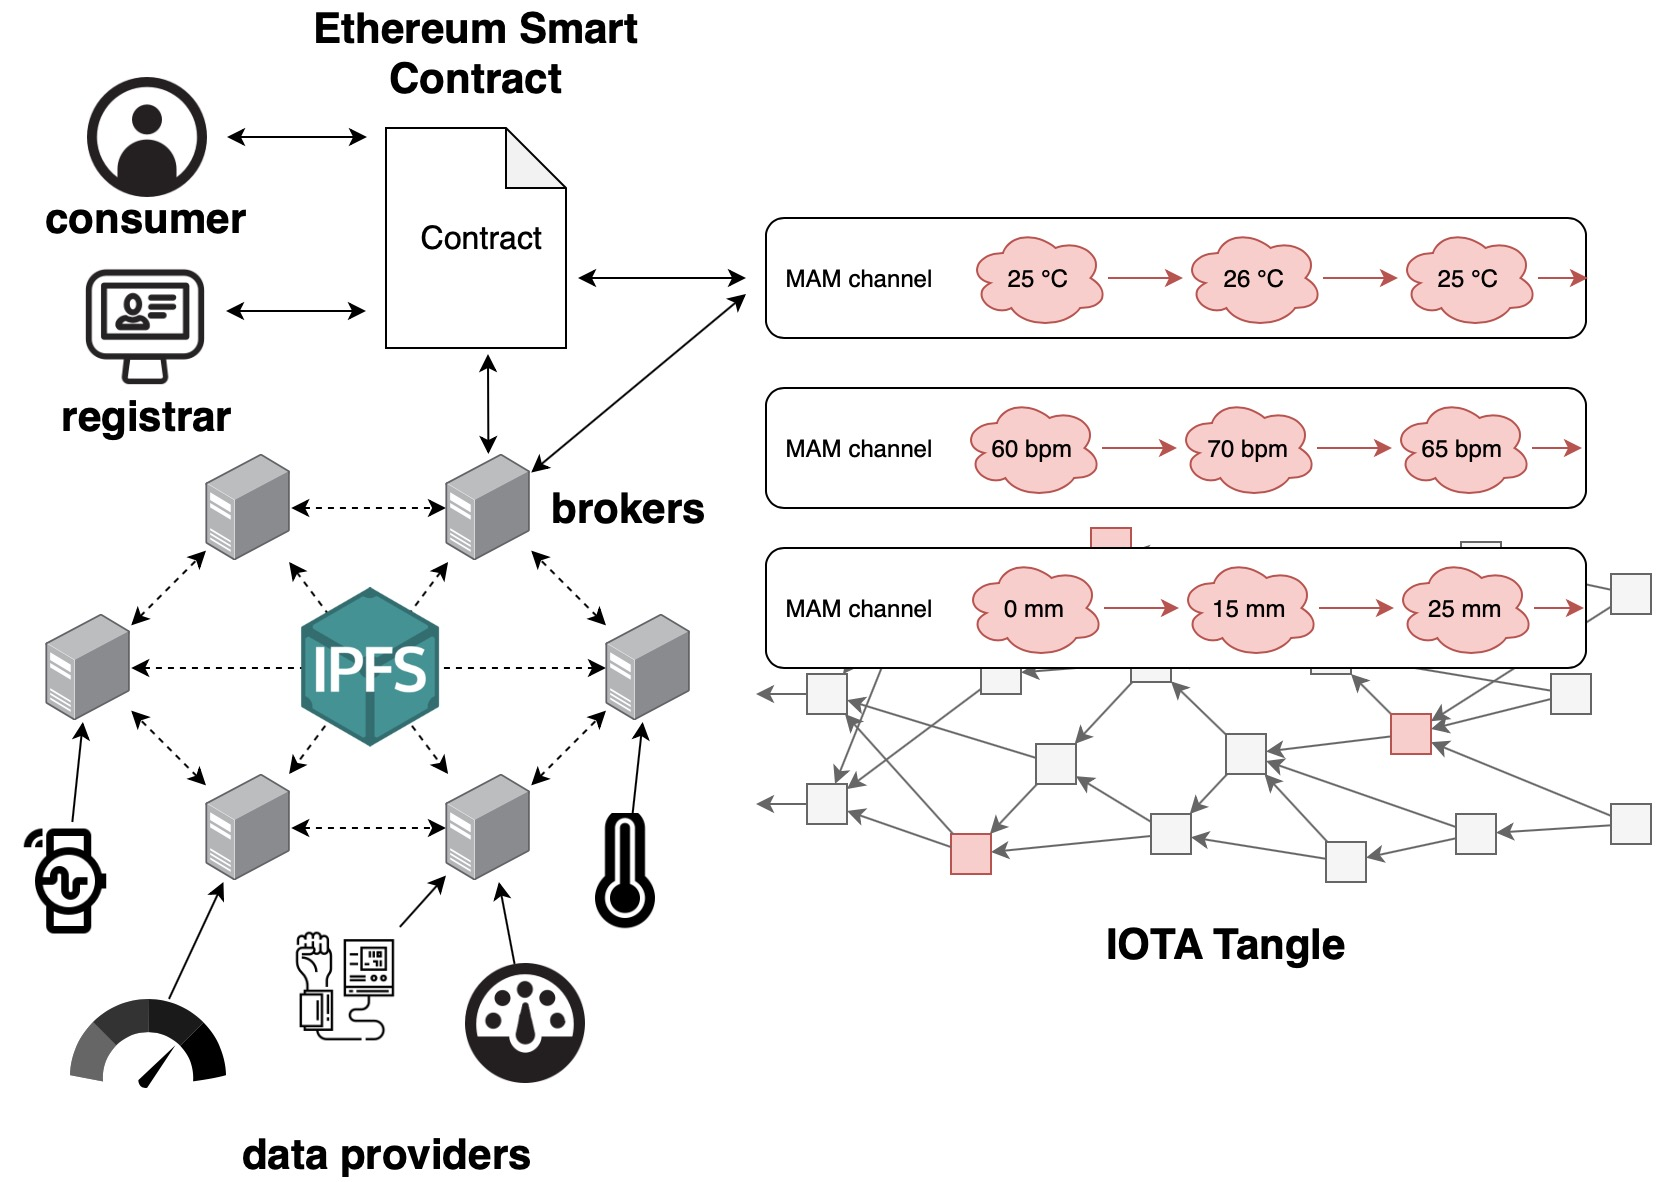
\includegraphics[width=0.4\textwidth]{system_design}
    \caption{The system design of a decentralized architecture which consists of a registrar, data providers, consumers and brokers.}
    \label{fig:system_design}
\end{figure}

\subsection{Components}
\subsubsection{Masked Authenticated Messaging}
MAM is a second layer data communication protocol built on the IOTA peer-to-peer network infrastructure, the Tangle. It resolves the challenges to publish encrypted streaming data to the distributed ledgers with session keys to channel, which indicates that each address is derived from its previous one. In other words, with channel root (a.k.a., the first message of a channel) and its session key, all data becomes accessible and validatable. Furthermore, each user can create multiple channels as possible.

\subsubsection{Decentralized Identifiers}
The TangleID\cite{TangleID} is a self-sovereign identity system that does not require any third-party authority to verify an identity and its digital footprint. With it, the digital footprint is converted into digital assets under the principle of Decentralized Identifiers (DIDs)\cite{DID} defined by W3C. Posting DID documents on MAM makes TangleID a GDPR-Complianced system\cite{GDPR}. Every participant in the data marketplace registers on TangleID, hence one can easily verify data providers' identity to ensure the data persistency from data sources.

\subsubsection{Ethereum Smart Contract}
Smart contract is a protocol for formulating agreement on a DLT/blockchain that provides verification and execution of the contract. All conditions and states established in the contract are enforeced with transparency. The appearance of smart contracts meet different requirements of trading pattern.

\subsubsection{Blind Signature}
Blind signature\cite{blindSig} is used to prevent the situation that the a broker would stole data if a session key is not encryted. In fact, blind signature is a form of digital signature where the message is first "blinded" by a random "blinding factor", and then passed to a signer to confirm. The encrypted message, along with the blinding factor, can be later verified with the signer's public key.

\subsubsection{IPFS}
Inter-Planetary File system(IPFS)\cite{IPFS} is a peer-to-peer network for storing and accessing files, websites, applications, and data in a distributed file system which is maintained with all IPFS users. In our proposed architecture, brokers are responsible for publishing metadata to IPFS, including titles, data provider information and data preview to provide users with searching capabilities.

\section{\normalsize\textbf{Trading Model}}
In the following, we describe the data registration, production launching, product searching and trading process in detail where we use game theory to ensure the sustainability of our trading model. The whole process is defined in smart contracts which are easily traceable and irreversible.

\subsection{Participant Registration}
At the beginning, the registrar creates a Registration Contract, which maintains all participants' information, including their DID documents and public keys. Everyone can query others' public keys for validation but only registrars have permission to add new members. After registration, the launching and trading processes can begin.

\subsection{Launching and Searching Products}
To sell streaming data, a data provider needs to launch a new product on the data marketplace in advance. The data provider determines a trusted broker and asks the broker to create a new MAM channel and product contract. Each product has a product contract to record the participants, subscription price brokerage fee, quantity of data and trading process.

Brokers certify session keys as well. Only one session key can be signed for each product, so data providers cannot fake a session key to deceive consumers. To certify a session key $k$, the data provider first blinds the session key with broker's public key from Registration Contract and sends $Blind(k)$ to the broker. The broker signs it and returns the signature $Sign(Blind(k))$ back, then the data provider removes the blinding factor and obtains the broker's signature of the session key, $Sign(k)$, which is verifiable by consumers.

\begin{figure}[h]
    \centering
    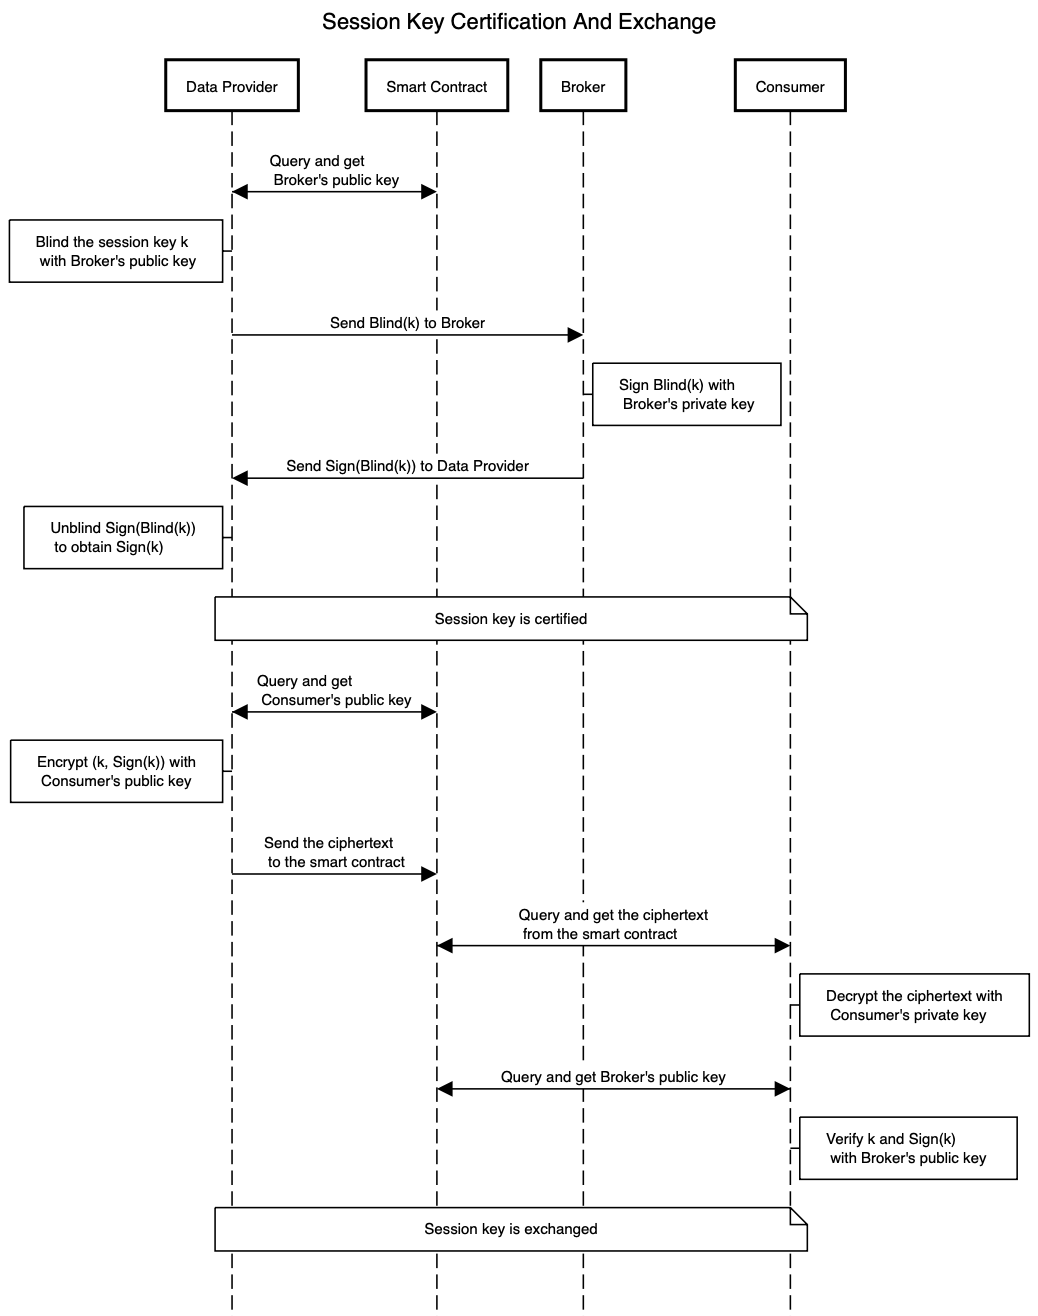
\includegraphics[width=0.5\textwidth]{key_certification_exchange}
    \caption{Session key certification with blind signature and session key exchange.}
    \label{fig:key_certification_exchange}
\end{figure}

The contract address and product description will be stored in a file which is uploaded to IPFS. Consumers can search the desired product by keywords or tags and then launch a trading process for interested products.

\subsection{Trading}
Once a consumer subscribes to certain streaming data that is generated pays a subscription fee to the purchase contract, he/she is added to the consumers list automatically by the smart contract.

Next, session key $k$ should be exchanged between the data provider and consumers. For each consumer, the data provider encrypts the session key and broker's signature with the consumer's public key and sends the ciphertext $Encrypt(k + Sign(k))$ to the purchase contract. Consumers can decrypt $Encrypt(k + Sign(k))$ to obtain and verify the session key $k$ and signature $Sign(k)$. Afterward, consumers can access data with session key on the MAM channel.

\subsection{Refunding}
It is probable that the streaming data sources are delayed or even interrupted after the consumers pay the subscription fee. To protect consumer rights, the subscription fee are not transferred to the data provider until data is generated and published to the MAM channel. If the expected data is not available, consumers can request refunds. We assume that a very small percentage of consumers in the product contract are irrational and/or malicious. Each consumer can vote for a refund at any time. If the ratio of consent votes of refunding is higher than the $threshold$ at the $i$th piece of data, the subscription fee is proportionally transferred to the data provider, broker and every consumer. The subscription fee can be prorated as below:

\begin{equation}
    F_{DataProvider}(i) = N price \frac{i-1}{M} (1-F_{b}) -F_{t}
\end{equation}

\begin{equation}
    F_{Broker}(i) = N price \frac{i-1}{M} F_{b} -F_{t}
\end{equation}

\begin{equation}
    F_{Consumer}(i) = price \frac{M-i+1}{M} -F_{t}
\end{equation}

where $price$ is the subscription price, $M$ is the number of expected data samples, $F_{b}$ (\%) is the brokerage fee which is expressed as a percentage, $F_{t}$ is the transaction fee of the smart contract, $N$ is the number of consumers in this contract.

To refund or withdraw subscription fees from the smart contract, the data provider, broker, and consumer send a transaction to execute the smart contract and are responsible for the transaction fee.

\subsection{Game Theory Evaluation}
Game Theory is a methodology to discuss strategic interaction among game players. We can ensure the sustainability of decentralized data marketplace by proving the existence of Nash Equilibrium at a certain acceptable range. Fan Liang et al\cite{SurveyBigDataPricing} listed several different types of game theory models in data pricing, and we employ repeated games which fits the scenario of data subscription to build our model.

Each consumer would pay subscription fee, $p_s$, each time they receive data from data provider. The sum of all the subscription fee paid to the data provider is denoted as $P_s$.

For every $n$ round, the data provider would pay $C_{maintain}$ to enhance the sensors that the data provider owns. We call this a maintenance period. Moreover, the value of data and the cost of maintenance will decrease as time passes, so we introduce a discounted factor $\beta$ to depict this phenomena.

Following assumptions are made:
\begin{enumerate}
    \item  We assume consumers are rational. \label{rational_man}
    \item  Each data provider is the sole provider of the product they produced. \label{monopoly}
    \item  Subscription fees only depends on data quality. \label{fee_vs_quality}
    \item  At least 51\% of consumers are in the same group which has complete information exchange.\label{51_in_group}
    \item  One of the consumers who has complete information exchange with other 51\% buyers has the ability to examine data quality. \label{1_in_51}
\end{enumerate}

According to \textbf{Assumption(\ref{rational_man})}, we learn that few consumers would take malicious actions in this system, since all the consumers are rational. \textbf{Assumption(\ref{monopoly})} implies each product is unique in the data marketplace. Therefore, each provider's behavior independently and the decision tree represents the behavior of only one data provider. From \textbf{Assumption(\ref{51_in_group})}, we derive that any consumer in that group launches voting for refund (i.e., the consumer announces the data quality is not acceptable) would succeed. \textbf{Assumption(\ref{1_in_51})}  implies if unacceptably low accuracy data are delivered to consumers, the examiner will spread this information out.


Based on the assumptions above, the discounted sum of payoff for our repeated game is
\begin{equation} \label{payoff}
    \sum_{i=0}^{m - 1}{\beta^{in}\cdot [(\sum_{j=0}^{n - 1} \beta^j \cdot P_s) - C_{maintain}]}
\end{equation}

Al-Fagih et al. presented\cite{DataPrice} the quality of data $P_s$ is sigmoid function of $P_r$, and based on rule of thumb $C_{maintain}$ is approximately an exponential function of $P_r$. We can substitute $P_s$ and $C_{maintain}$ with $P_r$ into Eq. (\ref{payoff}), then we can find out the Nash Equilibrium of repeated game.

To evaluate the behavior of the model we presented, first, we would express the function of $P_s$ and $C_{maintain}$ as functions of $P_r$ respectively. Therefore, the sum of subscription fee of all subscriber can be expressed as

\begin{equation} \label{sub_fee}
    P_s = R \frac{e^{a (P_r - b)}}{1 + e^{a (P_r - b)}}
\end{equation}

where $a$ and $b$ are tuning factors, and $R$ is the maximum data value.
And we would express the cost of maintenance as

\begin{equation} \label{C_mtn}
    C_{maintain} = ce^{P_r - d}
\end{equation}
Where $c$ and $d$ are tuning factors.

Substitute Eq. (\ref{sub_fee}) and Eq. (\ref{C_mtn}) into Eq. (\ref{payoff}). We can derive an equation illustrating the market mechanism of the subscription trading policy in the proposed decentralized data marketplace. First, data providers have weak motivation to operate their sensor in low accuracy, since the incentive of low quality data is much less than moderate quality data. Second, the great deficit at high accuracy is mostly derived by the rapid increasing of maintenance cost. Thus, if the maintenance fee to achieve decent data quality is under a fair price range, then data provider will automatically provide data with high data quality under our assumptions.

\section{\normalsize\textbf{Conclusion and Future Work}}
To our knowledge, this paper is the first attempt to construct fully decentralized data marketplaces with strong data integrity and transparency in mind.
The data auction process is a data trading mechanism and an economically-driven scheme that establishes corresponding prices of data products through bidding process between consumers and providers. While there have been various auction models\cite{BigPicDataMarket} in several areas, only few researches focus on third-party auction platforms. Our proposed decentralized data marketplace protects the privacy of participants which reveals the minimum information for validation and reduces the suspicion of trust to centralized parties or auctioneers. However, the auction process between multiple participants, analysis of potential threats and an overall game theory evaluation are still critical issues that need to be resolved.


% ---- Bibliography ----
\bibliographystyle{IEEEtran}
\bibliography{references}
\end{document}
